\documentclass{article}

\usepackage{geometry}
 \geometry{
 a4paper,
 total={170mm,257mm},
 left=20mm,
 top=20mm
 }
\usepackage{float}
\usepackage{graphicx}
\usepackage{indentfirst}
\usepackage{hyperref}
\graphicspath{ {./images/} }

\begin{document}
	\section{Analisis Hasil Model CapsNet}
	\begin{itemize}
	
	    \begin{figure}[H]
			\centering
			
\includegraphics[scale=1]{analisis model/final_acc.eps}
		\end{figure}
	
		\item Grafik akurasi data validasi menunjukkan fluktuasi besar di 5 \textit{epoch} pertama, karena nilai-nilai awal pada matriks beban model bersifat acak sehingga model belum bisa membuat prediksi dengan akurat. Untuk \textit{epoch} ke 10 dan seterusnya, akurasi validasi model sudah stabil dengan akurasi sekitar 90 persen. Akurasi tes yang hanya sedikit kurang dari akurasi validasi akhir membuktikan bahwa model dapat generalisasi dengan baik pada data yang belum pernah dilihatnya.
		
	    \begin{figure}[H]
			\centering
			
\includegraphics[scale=1]{analisis model/final_acc_norm.eps}
		\end{figure}
		
		\item Bila proses normalisasi diaplikasikan ke gambar masukan, akurasi validasi model sedikit berkurang. Normalisasi pada gambar masukan berguna pada model CNN sebab model CNN belajar dengan secara terus-menerus menambahkan gradien \textit{error vector} dikalikan dengan \textit{learning rate} ke berbagai matriks beban. Bila vektor masukan tidak dinormalisasi, maka jarak distribusi nilai-nilai fitur akan berbeda untuk setiap fitur, sehingga hasil kurang maksimal. Namun, tampaknya normalisasi tidak membantu meningkatkan performa model CapsNet, melainkan sedikit menurunkan performanya.
		
	    \begin{figure}[H]
			\centering
			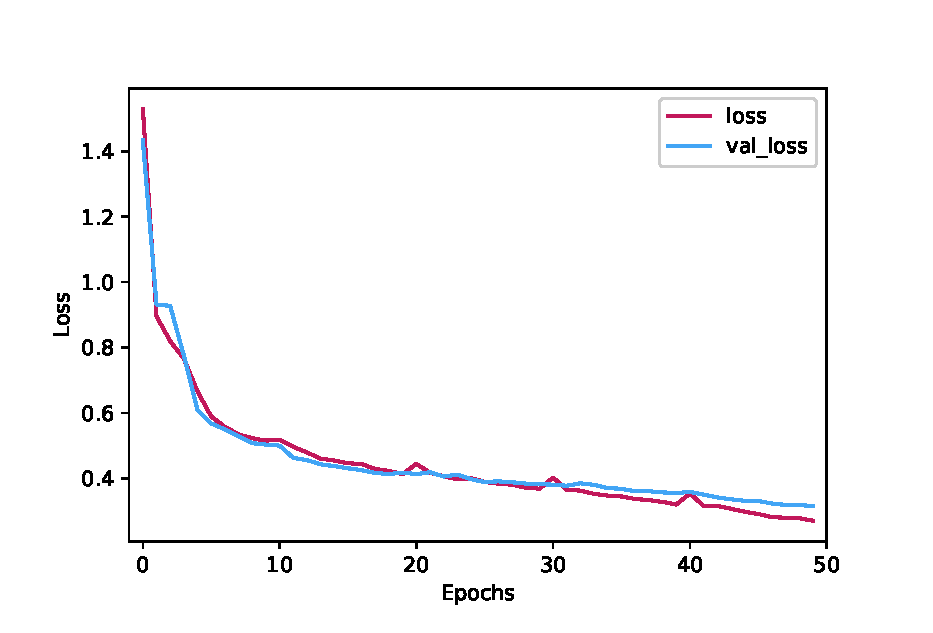
\includegraphics[scale=1]{analisis model/final_loss.eps}
		\end{figure}
		
		\item Nilai fungsi \textit{loss} dari model terlihat menurun drastis pada 10 \textit{epoch} pertama, lalu menurun secara perlahan di \textit{epoch-epoch} berikutnya. \textit{Loss} pada model ketika latihan dan\textit{loss} pada validasi terlihat mendekati satu sama lain, membuktikan bahwa model tidak mengalami \textit{overfit}.
		
		\begin{figure}[H]
			\centering
			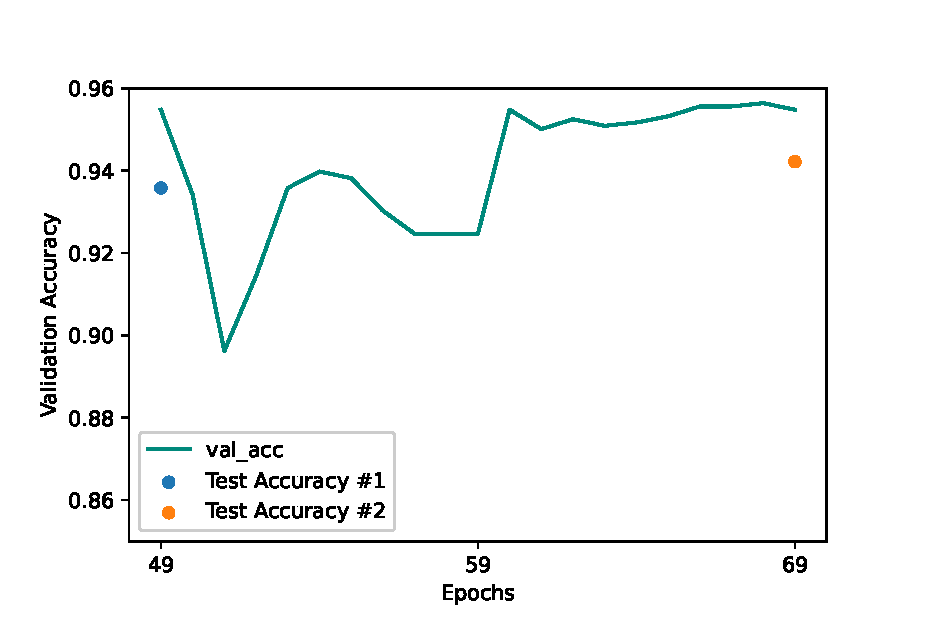
\includegraphics[scale=1]{analisis model/covid_learn_acc.eps}
		\end{figure}
	
		\item Akurasi validasi untuk khusus kasus-kasus COVID-19 terlihat fluktuatif sampai \textit{epoch} ke 60. Pada \textit{epoch} ke 61 dan seterusnya, kami mencoba memasukan lebih banyak gambar-gambar kasus COVID-19 untuk menambahkan informasi yang didapat oleh model. Hasilnya adalah akurasi validasi model mulai lebih stabil di sekitar 95 persen, dan akurasi tes model untuk kasus-kasus COVID-19 tercatat dengan akurasi sekitar 94 persen.
		
		\begin{center}
			\begin{tabular}{|c|c|c|c|}
				\hline
				& \textit{Normal (Predicted)} & \textit{Pneumonia (Predicted)} & \textit{Covid (Predicted)} \\
				\hline
				\textit{Normal (Actual)} & 292 & 24 & 1 \\
				\hline
				\textit{Pneumonia (Actual)} & 30 & 821 & 3 \\
				\hline
				\textit{Covid (Actual)} & 4 & 10 & 77 \\
				\hline
			\end{tabular}
		\end{center}
	
		\item Hasil \textit{confusion matrix} model akhir menunjukkan bahwa model dapat dengan tepat mengklasifikasikan 77 dari 91 kasus COVID-19. Dari 1171 kasus-kasus yang bukan COVID-19, model hanya mengklasifikasikan secara salah 4 kasus sebagai kasus COVID-19. 
	
		\begin{center}
			\begin{tabular}{|c|c|c|c|}
				\hline
				& \textit{Precision} & \textit{Recall} & \textit{F1-score} \\
				\hline
				\textit{Normal} & 0.90 & 0.92 & 0.91 \\
				\hline
				\textit{Pneumonia} & 0.96 & 0.96 & 0.96 \\
				\hline
				\textit{Covid} & 0.95 & 0.85 & 0.90 \\
				\hline
				\hline
				\textit{Macro Avg} & 0.94 & 0.91 & 0.92 \\
				\hline
				\textit{Weighted Avg} & 0.94 & 0.94 & 0.94 \\
				\hline
				\hline
				\textit{Accuracy} & \multicolumn{3}{|c|}{0.94} \\
				\hline
			\end{tabular}
		\end{center}
	
		\item Akurasi keseluruhan model tercantum pada angka 94 persen. \textit{Macro average} menghitung nilai rata-rata \textit{precision}, \textit{recall}, dan \textit{F1-score} dari tiap kelas. \textit{Weighted average} menambahkan nilai \textit{precision}, \textit{recall}, dan \textit{F1-score} masing-masing kelas dengan dikalikan beban yang tergantung dengan jumlah kasus benar dari tiap kelas. Terlihat bahwa \textit{weighted average} dari \textit{precision}, \textit{recall}, dan \textit{F1-score} bernilai konsisten dengan akurasi keseluruhan, yaitu 94 persen.
		
	\end{itemize}
\end{document}